\section{Popper-compliant Papers}
\label{sec:popper-compliant-papers}

We have produced four Popper-compliant papers, as shown in
Table~\ref{table:papers}. These papers follow the reader/reviewer sample
workflow outlined in~\cite{jimenez:ipdpsw17-popper} and shown in
Figure~\ref{fig:workflow}. For the visualization component (1), we use Jupyter
notebooks. The notebooks themselves are versioned with Git and users interact
with local copies by cloning the repository and launching a Jupyter Docker
container. The paper is written in \LaTeX and built with a Docker container.
For the code component (2), both the source code for the system itself and the
deploy/experiment code is stored on GitHub. When running experiments, we use
Docker containers to isolate libraries and binaries. For the multi-node
component (3), we use CloudLab machines and Ansible to script deployment and
experiment orchestration. For the data set components (4), we use GitHub to
store results files; our inputs and results are small enough that we do no need
a larger capacity.  GitHub allows files up to 50MB and stores data on S3.

Our experiments start with a baseline. To describe the process, we reference
our
ceph-popper-template\footnote{https://github.com/michaelsevilla/ceph-popper-template}
set up on CloudLab. Users setup SSH keys and deploy CloudLab nodes using our
CephFS Profile\footnote{https://www.cloudlab.us/p/CephFS/CephFS-HEP}.  The
profile has the nodes automatically install Docker on bootup using our
install\footnote{https://github.com/michaelsevilla/ceph-popper-template/blob/master/hardware/cloudlab/\-install.sh}
script. After the nodes finish booting ({\it i.e.}  their status on the
CloudLab GUI is READY), users push SSH keys using a convenience
script\footnote{https://raw.githubusercontent.com/michaelsevilla/ceph-popper-template/master/hardware/cloudlab/pushkeys.sh}.

The deploy code is based on
ceph-ansible\footnote{https://github.com/ceph/ceph-ansible/wiki}, a tool that
configures hardware and software for Ceph. We forked the project and made it
less dependent on Python. To run an experiment, users log into the head node
and clone the ceph-popper-template repository. This repository has submodules
that point to ceph-ansible and our own custom roles; configuration files for
our Ceph setup; and helper scripts written in bash that deploy Ceph and run the
benchmarks.  For more information on the Ceph template, see the
README\footnote{https://github.com/michaelsevilla/ceph-popper-template} and for
more information on the baseline and pipelines terminology, see the Popper
Convention quickstart\footnote{http://falsifiable.us/}. 

\begin{figure}[tb] 
  \centering
  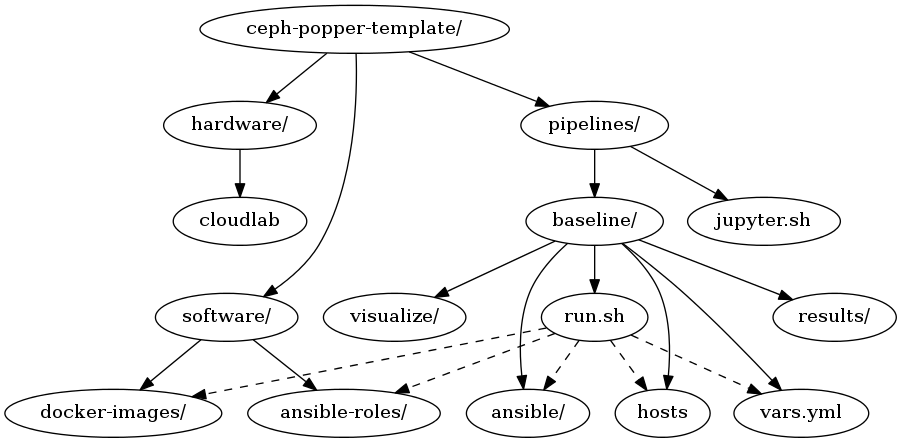
\includegraphics[width=1\linewidth]{./figures/expdir.png}
  \caption{Organization of our experiment directories. \texttt{baseline/} is an
example experiment and contains scripts populated with the Popper CLI. The
\texttt{run.sh} script uses many directories and files to setup and run
experiments, as indicated by the dashed lines.}
  \label{fig:expdir}
\end{figure}

An outline of this organization is shown in Figure~\ref{fig:expdir}, where
solid lines are directory links and dashed lines indicate which directories a
script uses.  A sample experiment is in the \texttt{baseline/} directoriy,
which was created using the Popper CLI. Users configure their cluster by
specifying hostnames and login user names in the \texttt{hosts} file.  Users
also specify the Ceph services that should be deployed using the
\texttt{ansible/}
directory\footnote{https://github.com/michaelsevilla/ceph-popper-template/tree/master/pipelines/baseline/ansible}.
This directory has code for deploying Ceph and its components, where the
\texttt{*.yml} files are Ansible playbooks that start and configure components:
\texttt{ceph.yml} starts Ceph and can be modified to specify which daemons to
launch, \texttt{cleanup.yml} tears Ceph down, and \texttt{monitor.yml} starts
daemons that monitor performance.  High level configurations are in the
\texttt{vars.yml} file.  We separate these components into different playbooks
so users can mix and match Ceph services.  Similarly, the workloads directory
has scripts for running the baseline benchmarks. The other files and
directories are Ansible configuration files used by the playbooks. We have
posted a tutorial on our
blog\footnote{http://programmability.us/mantle/blog2-ceph} to guide users
through this setup. When complete, users execute the \texttt{run.sh} to start
the job.


